\everymath{\displaystyle}
\documentclass{beamer}
% \documentclass[handout]{beamer}

%\usepackage[pdftex]{color,graphicx}
\usepackage{amsmath,amssymb,amsfonts}

\mode<presentation>
{
  % \usetheme{Darmstadt}
  % \usetheme[hideothersubsections]{Hannover}
  % \usetheme[hideothersubsections]{Goettingen}
  \usetheme[hideothersubsections, right]{Berkeley}

  \usecolortheme{seahorse}
  % \usecolortheme{dolphin}
  \usecolortheme{rose}
  % \usecolortheme{orchid}

  \useinnertheme[shadow]{rounded}

  \setbeamercovered{transparent}
  % or whatever (possibly just delete it)
}

\mode<handout>{
  \setbeamercolor{background canvas}{bg=black!5}
  \usepackage{pgfpages}
  \pgfpagesuselayout{4 on 1}[a4paper,border shrink=5mm, landscape]
}

\usepackage[brazilian]{babel}
% or whatever

% \usepackage[latin1]{inputenc}
\usepackage[utf8]{inputenc}
% or whatever

\usepackage{times}
%\usepackage[T1]{fontenc}
% Or whatever. Note that the encoding and the font should match. If T1
% does not look nice, try deleting the line with the fontenc.


\title%[] % (optional, use only with long paper titles)
{Estrutura do trabalho científico II}

\subtitle
{Forma} % (optional)

\author%[] % (optional, use only with lots of authors)
{Felipe Figueiredo}% \and S.~Another\inst{2}}
% - Use the \inst{?} command only if the authors have different
%   affiliation.

\institute[INTO] % (optional, but mostly needed)
{Instituto Nacional de Traumatologia e Ortopedia
}
  % \inst{1}%
  % Department of Computer Science\\
  % University of Somewhere
  % \and
  % \inst{2}%
  % Department of Theoretical Philosophy\\
  % University of Elsewhere}
% - Use the \inst command only if there are several affiliations.
% - Keep it simple, no one is interested in your street address.

\date%[] % (optional)
{}

% \subject{Talks}
% This is only inserted into the PDF information catalog. Can be left
% out. 



% If you have a file called "university-logo-filename.xxx", where xxx
% is a graphic format that can be processed by latex or pdflatex,
% resp., then you can add a logo as follows:

\pgfdeclareimage[height=1.6cm]{university-logo}{../logo}
\logo{\pgfuseimage{university-logo}}



% Delete this, if you do not want the table of contents to pop up at
% the beginning of each subsection:
\AtBeginSubsection[]
%\AtBeginSection[]
{
  \begin{frame}<beamer>{Sumário}
    \tableofcontents[currentsection,currentsubsection]
  \end{frame}
}


% If you wish to uncover everything in a step-wise fashion, uncomment
% the following command: 

% \beamerdefaultoverlayspecification{<+->}


\begin{document}

\begin{frame}
  \titlepage
\end{frame}

\begin{frame}{Sumário}
  \tableofcontents
  % You might wish to add the option [pausesections]
\end{frame}


%% Template
% \section{}

% \subsection{}

% \begin{frame}{}
%   \begin{itemize}
%   \item 
%   \end{itemize}
% \end{frame}

% \begin{frame}
%   \begin{columns}
%     \begin{column}{5cm}
%     \end{column}
%     \begin{column}{5cm}
%     \end{column}
%   \end{columns}
% \end{frame}

% \begin{frame}{}
%   \includegraphics[height=0.4\textheight]{file1}
%   \includegraphics[height=0.4\textheight]{file2}
%   \includegraphics[height=0.4\textheight]{file3}
%   \begin{figure}
%     \caption{}
%   \end{figure}
% \end{frame}

% \begin{frame}{}
%   \begin{definition}
%   \end{definition}
%   \begin{example}
%   \end{example}
%   \begin{block}{Exercício}
%   \end{block}
% \end{frame}

% \section{Elementos pré-textuais}

\section{Discussão da aula passada}

% \subsection{Discussão da aula passada}

\begin{frame}{Discussão da aula passada}
  \begin{block}{}
    Discussão da leitura obrigatória da aula passada
  \end{block}
\end{frame}

\section{Formatação}

\subsection{Gerais}

\begin{frame}{Identifique os erros...}
  \begin{center}
    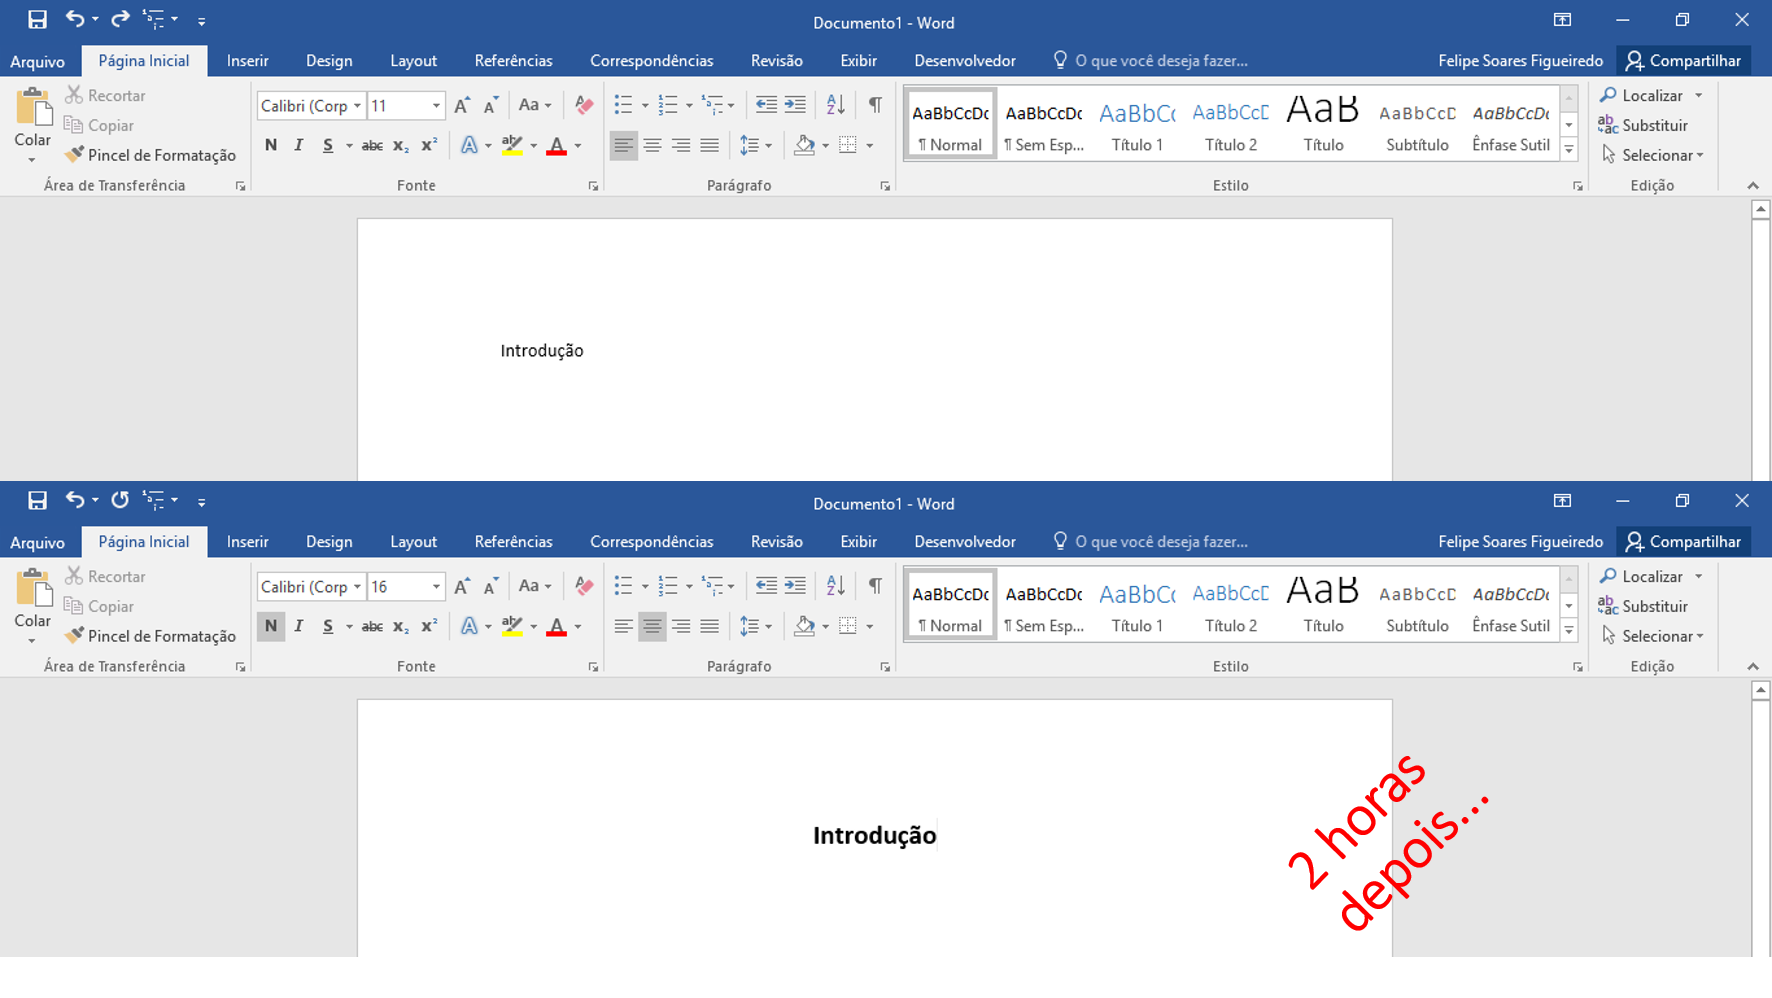
\includegraphics[width=1.2\textwidth]{EstruturaII/intro}
  \end{center}
\end{frame}

\begin{frame}
  \begin{enumerate}
    \footnotesize
  \item A formatação foi feita manualmente
    \bigskip
  \item Não foi seguida a Norma ABNT para o título de seção primária
    \begin{itemize}
      \tiny
    \item centralizado
    \item sem numeração
    \item capitalização comum (caixa baixa)
    \item já mencionei que foi feita manualmente?
    \end{itemize}
    \bigskip
  \item 2h?? ({\em come on}...)
  \end{enumerate}
\end{frame}

\begin{frame}{Padronização da página}
  \begin{itemize}
    \footnotesize
  \item Papel: A4
    \medskip
  \item Fonte: Arial (ou Times) 12
    \medskip
  \item Espaçamento 1,5
    \medskip
  \item Margens
    \begin{itemize}
      \tiny
    \item superior: 3cm
    \item inferior: 2cm
    \item esquerda: 3cm
    \item direita: 2cm
    \end{itemize}
  \end{itemize}
\end{frame}

\begin{frame}{Numeração de seções}
  \begin{center}
    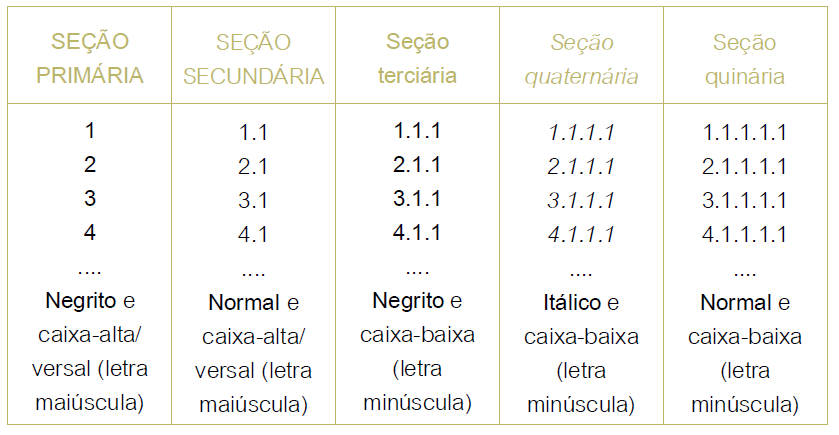
\includegraphics[width=\textwidth]{EstruturaII/secoes}
  \end{center}

  \vfill
  \scriptsize
  \hfill Fonte: Prodanov, 2013
\end{frame}

\begin{frame}{}
  \begin{block}{Lembre-se!}
    \footnotesize
    Cada instituição tem autonomia para definir sua própria norma interna
  \end{block}
\end{frame}

\subsection{Capa e folha de rosto}

\begin{frame}{\scriptsize Capa}
  \scriptsize
  A capa deve identificar claramente:

  \bigskip
  \begin{itemize}
    \footnotesize
  \item Instituição (nome, sigla, logotipo opcional)
    \bigskip
  \item Nome(s) do(s) pesquisador(es)
    \bigskip
  \item Nome(s) do(s) orientador(es)
    \bigskip
  \item Data (ano, e talvez também o mês)
  \end{itemize}
\end{frame}

\begin{frame}
  \begin{exampleblock}{Exemplo}
    \begin{center}
      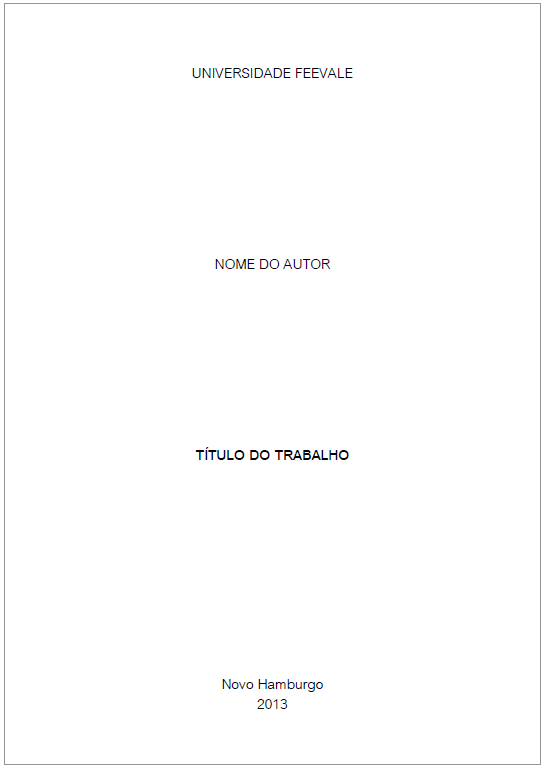
\includegraphics[height=0.8\textheight]{EstruturaII/capa}
    \end{center}
  \end{exampleblock}

  \vfill
  \scriptsize
  \hfill Fonte: Prodanov, 2013
\end{frame}

\begin{frame}{\scriptsize Folha de rosto}
  \scriptsize
  A folha de rosto deve identificar claramente:
  \bigskip
  \begin{itemize}
    \footnotesize
  \item Instituição (nome, sigla)
    \bigskip
  \item Nome(s) do(s) autor(es)
    \bigskip
  \item Nome(s) do(s) orientador(es)
    \bigskip
  \item Data (ano, e talvez também o mês)
    \bigskip
  \item Natureza e objetivo
  \end{itemize}
\end{frame}

\begin{frame}
  \begin{exampleblock}{Exemplo}
  \begin{center}
    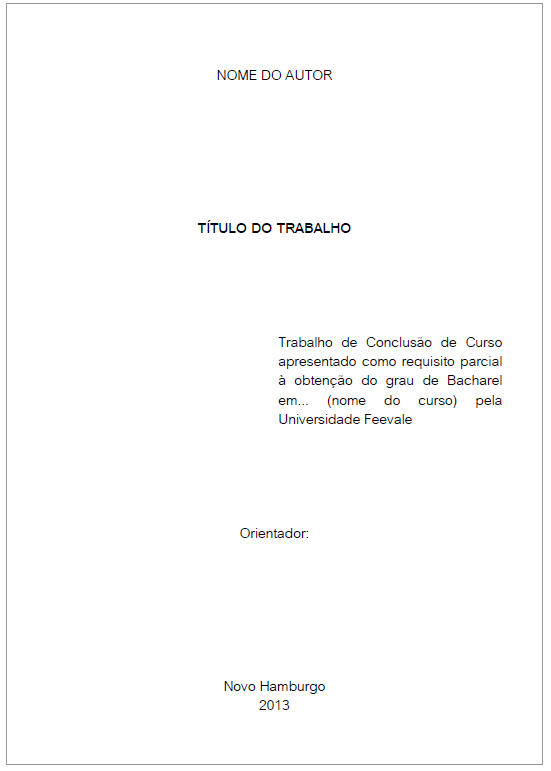
\includegraphics[height=0.8\textheight]{EstruturaII/rosto}
  \end{center}
\end{exampleblock}
  \vfill
  \scriptsize
  \hfill Fonte: Prodanov, 2013
\end{frame}

% \begin{frame}{INTO}
%   Exemplos: Projeto e Dissertação
% \end{frame}

\begin{frame}{\scriptsize INTO: Capa da Dissertação}
  \begin{exampleblock}{Exemplo}
    \begin{center}
      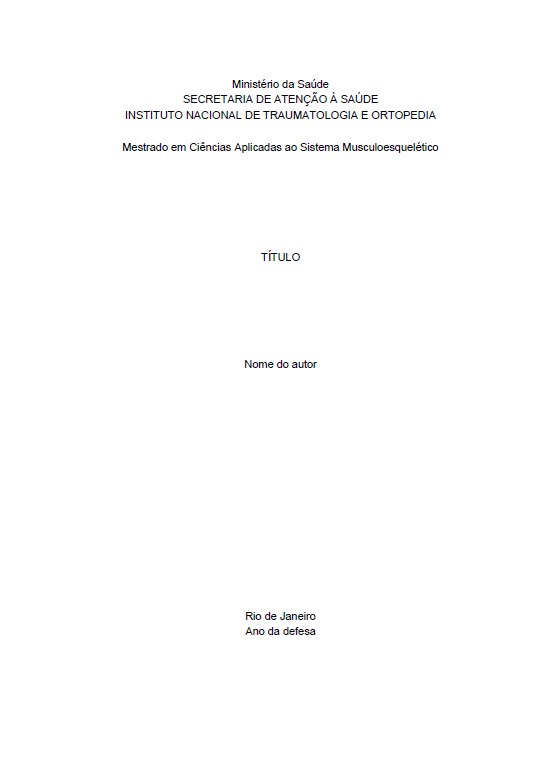
\includegraphics[height=.8\textheight]{EstruturaII/dirce}
    \end{center}
  \end{exampleblock}
\end{frame}

\begin{frame}{\scriptsize INTO: Capa do Seminário Discente (projeto)}
  \begin{exampleblock}{Exemplo}
    \begin{center}
      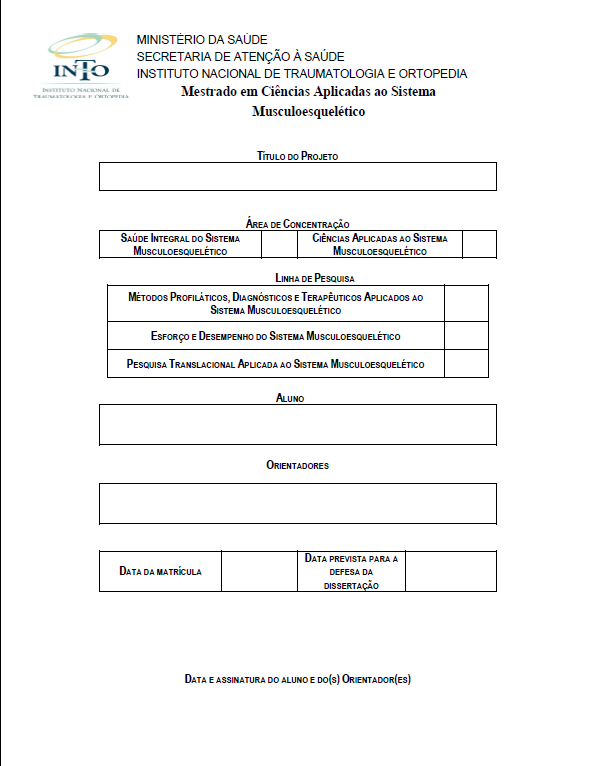
\includegraphics[height=.8\textheight]{EstruturaII/projeto}
    \end{center}
  \end{exampleblock}
\end{frame}

\subsection{Objetos visuais}

% \begin{frame}{Quadros e Tabelas}
%   \begin{itemize}
%     \footnotesize
%   \item Quadro -- informações qualitativas
%     \footnote{\scriptsize Não é determinado na norma ABNT, não é consenso nas PGs}
%     \begin{itemize}
%       \scriptsize
%     \item Fechado em todas as bordas
%     \item Legenda acima
%     \item Meta-informações abaixo
%     \item Fonte ligeiramente menor que o texto
%     \end{itemize}
%     \bigskip
%   \item Tabela -- informações quantitativas e resultados
%     \begin{itemize}
%       \scriptsize
%     \item Aberto nas bordas laterais
%     \item Legenda acima
%     \item Meta-informações abaixo
%     \item Fonte ligeiramente menor que o texto
%     \end{itemize}
%     \bigskip
%   \item \alert{\bf Obrigatório}
%     \begin{itemize}
%       \scriptsize
%     \item Conter informação suficiente para compreensão ({\tiny sem leitura do texto})
%     \item Sempre referenciar no texto
%     \end{itemize}
%   \end{itemize}

%   \vfill
%   \scriptsize
%   \hfill \href{http://www.biblioteca.fsp.usp.br/~biblioteca/guia/i_cap_04.htm}
%   {Guia de Apresentação de Teses -- FSP/USP}

%   \hfill \href{https://biblioteca.ibge.gov.br/index.php/biblioteca-catalogo?view=detalhes&id=223907}
%   {Normas de apresentação tabular -- IBGE}
% \end{frame}

% \begin{frame}{Quadros e Tabelas}
%   \begin{columns}
%     \begin{column}{5cm}
%       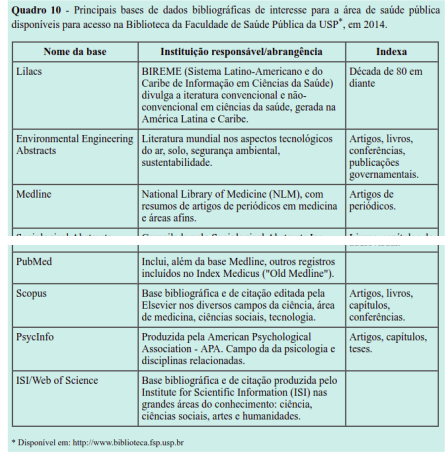
\includegraphics[width=\textwidth]{EstruturaII/obj-quadro}
%     \end{column}
%     \begin{column}{5cm}
%       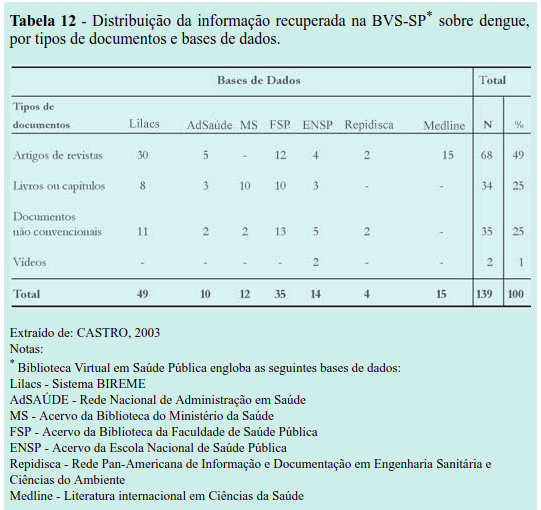
\includegraphics[width=\textwidth]{EstruturaII/obj-tabela}
%     \end{column}
%   \end{columns}

%   \vfill
%   \scriptsize
%   \hfill \href{http://www.biblioteca.fsp.usp.br/~biblioteca/guia/i_cap_04.htm}
%   {Guia de Apresentação de Teses -- FSP/USP}
% \end{frame}

\begin{frame}{Quadros}
  \begin{columns}%[t,onlytextwidth]
    \begin{column}{.5\textwidth}
      \begin{itemize}
        \scriptsize
      \item Quadro -- informações qualitativas ({\tiny literatura\footnote[frame]{\scriptsize Não é determinado na norma ABNT, não é consenso nas PGs}?})
        \begin{itemize}
          \tiny
        \item Fechado -- todas as bordas
        \item Legenda acima do objeto
        \item Meta-informações abaixo
        \item Fonte ligeiramente menor que o texto
        \end{itemize}
        \bigskip
      \item \alert{\bf Obrigatório}
        \begin{itemize}
          \tiny
        \item Conter informação suficiente para compreensão ({\tiny sem leitura do texto})
        \item Sempre referenciar no texto
        \end{itemize}
      \end{itemize}
    \end{column}
    \begin{column}{.5\textwidth}
      \visible<2>{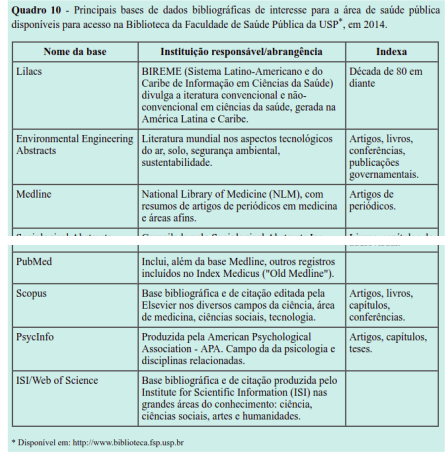
\includegraphics[height=.9\textheight]{EstruturaII/obj-quadro}}
    \end{column}
  \end{columns}

  \vfill
  \scriptsize
  \hfill \href{http://www.biblioteca.fsp.usp.br/~biblioteca/guia/i_cap_04.htm}
  {Guia de Apresentação de Teses -- FSP/USP}
\end{frame}

\begin{frame}{Tabelas}
  \begin{columns}
    \begin{column}{.5\textwidth}
  \begin{itemize}
    \scriptsize
  \item Tabela -- informações quantitativas e resultados
    \begin{itemize}
      \tiny
    \item Aberto nas bordas laterais
    \item Legenda acima do objeto
    \item Meta-informações abaixo
    \item Fonte ligeiramente menor que o texto
    \end{itemize}
    \bigskip
  \item \alert{\bf Obrigatório}
    \begin{itemize}
      \tiny
    \item Conter informação suficiente para compreensão ({\tiny sem leitura do texto})
    \item Sempre referenciar no texto
    \end{itemize}
  \end{itemize}
    \end{column}
    \begin{column}{.5\textwidth}
      \visible<2>{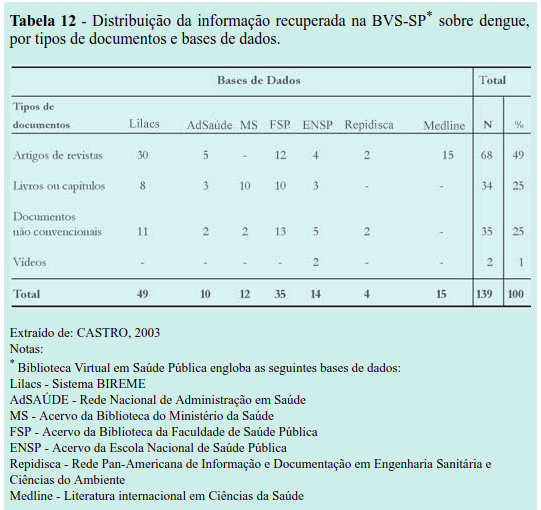
\includegraphics[height=.83\textheight]{EstruturaII/obj-tabela}}
    \end{column}
  \end{columns}

  \vfill
  \scriptsize
  \hfill \href{http://www.biblioteca.fsp.usp.br/~biblioteca/guia/i_cap_04.htm}
  {Guia de Apresentação de Teses -- FSP/USP}
\end{frame}

\begin{frame}{Figuras}
  \begin{itemize}
    \footnotesize
  \item Denominação genérica -- {\scriptsize imagens, gráficos, diagramas,} ...
  \item Legenda abaixo do objeto
    \bigskip
  \item \alert{\bf Obrigatório}
    \begin{itemize}
      \scriptsize
    \item Conter informação suficiente para compreensão ({\tiny sem leitura do texto})
    \item Sempre referenciar no texto
    \end{itemize}
  \end{itemize}
\end{frame}

\section{Sumários}

\subsection{Sumário do Projeto}

\begin{frame}{Sumário do projeto}
  \begin{itemize}
  \item Utilizar as ferramentas automáticas do software escolhido
    (Word, LibreOffice, \LaTeX, etc.)
  \item Formatar seções selecionando os {\bf estilos de texto}
    (ex. Título 1, Título 2, \ldots)
  \item \alert{Nunca} formatar seções manualmente! (vide cap {\bf 9})
  \item Indicar seções primárias, secundárias e terciárias
  \item (ABNT) Primárias em caixa alta, secundárias (em diante)
    capitalizadas
  \end{itemize}
\end{frame}

\begin{frame}{Exemplo}
  \begin{center}
    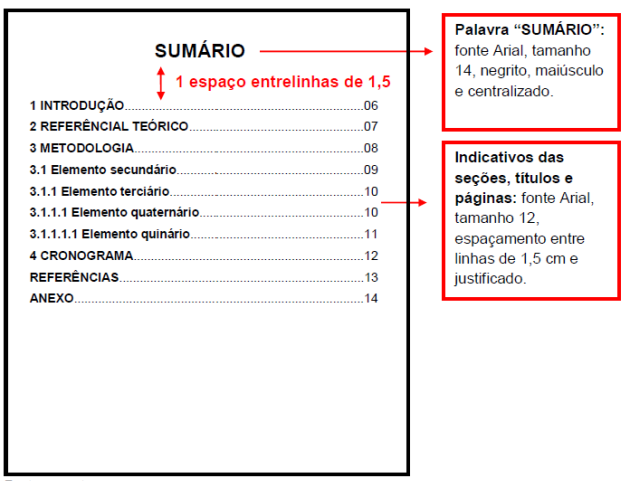
\includegraphics[height=0.8\textheight]{EstruturaII/sumario}
  \end{center}

  Fonte: \url{http://fio.edu.br/manualtcc/co/4_Sumario.html}
\end{frame}

\subsection{Lista de abreviaturas}

\begin{frame}{Lista de abreviaturas}
  \begin{itemize}
  \item Indicar \alert{todas} as abreviaturas utilizadas no texto
    (mesmo que uma única vez)
  \item Ordem alfabética das abreviaturas
  \item (ABNT) Sigla em caixa alta, significado capitalizado
  \end{itemize}
\end{frame}

\begin{frame}{Exemplo}
  \begin{center}
    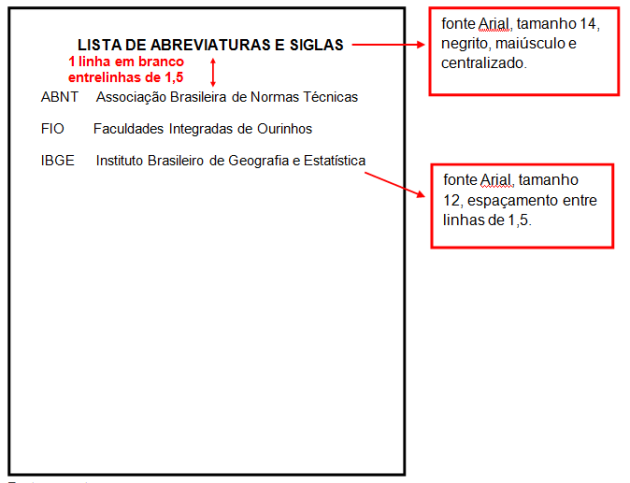
\includegraphics[height=0.8\textheight]{EstruturaII/lista_abreviaturas}
  \end{center}

  Fonte: \url{http://fio.edu.br/manualtcc/co/15_Lista_de_abreviaturas.html}
\end{frame}

\subsection{Listas de Figuras e Tabelas}

\begin{frame}{Listas de Figuras e de Tabelas}
  \begin{itemize}
  \item Legendas das figuras e tabelas, com o número de página em que
    aparecem
  \item Utilizar ferramentas automáticas (Inserir Figura/Tabela,
    Propriedades/Legenda).
  \item (opcional) versão resumida da legenda, caso muito longa
  \end{itemize}
\end{frame}

\begin{frame}{Exemplo}
  \begin{center}
    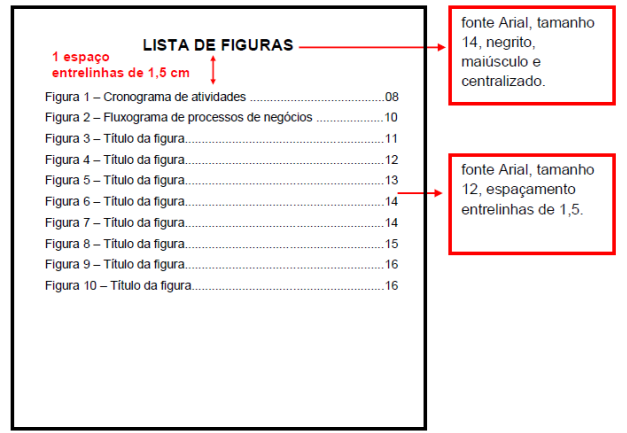
\includegraphics[height=0.8\textheight]{EstruturaII/lista_figuras}
  \end{center}

  Fonte: \url{http://fio.edu.br/manualtcc/co/13_Lista_de_ilustracoes.html}
\end{frame}

\subsection{Tutorial}

\begin{frame}{Tutorial}
  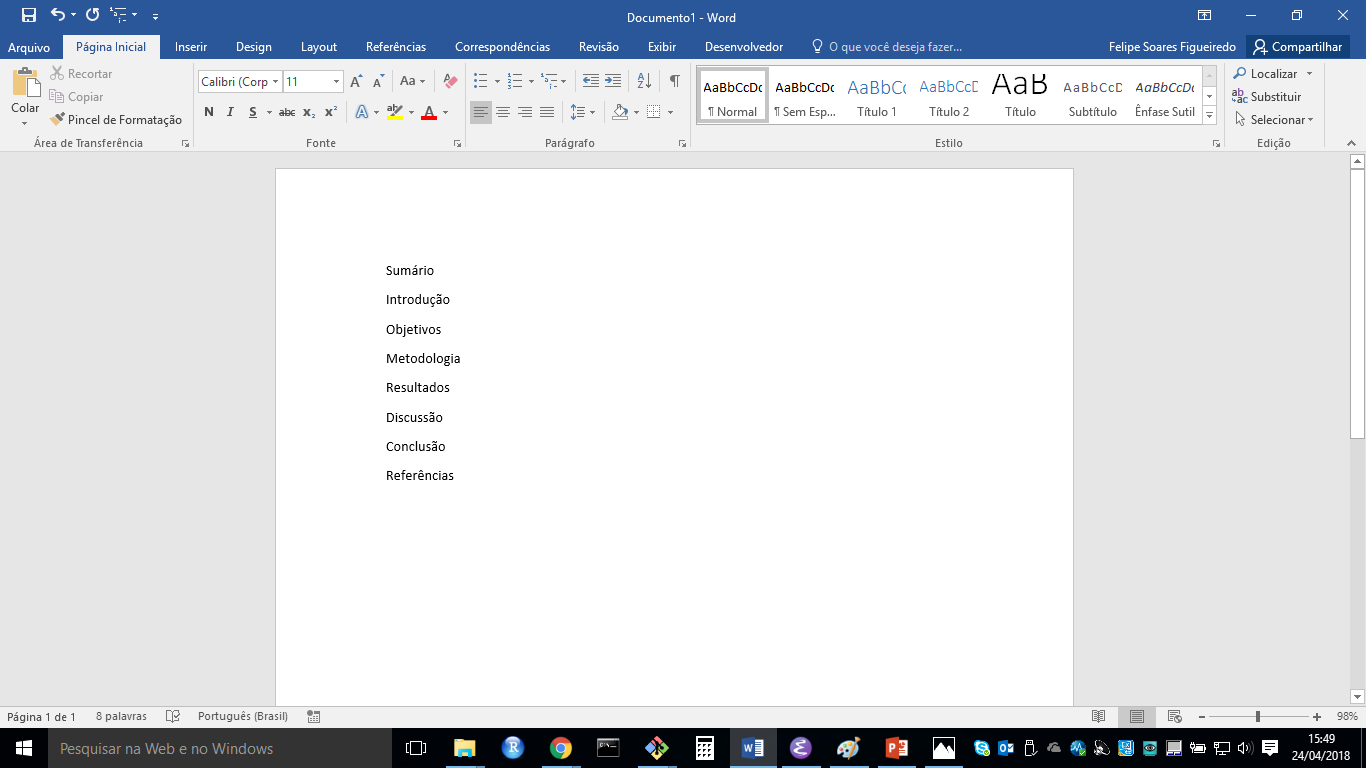
\includegraphics[height=0.9\textheight]{EstruturaII/sumario1}
\end{frame}

\begin{frame}{Tutorial}
  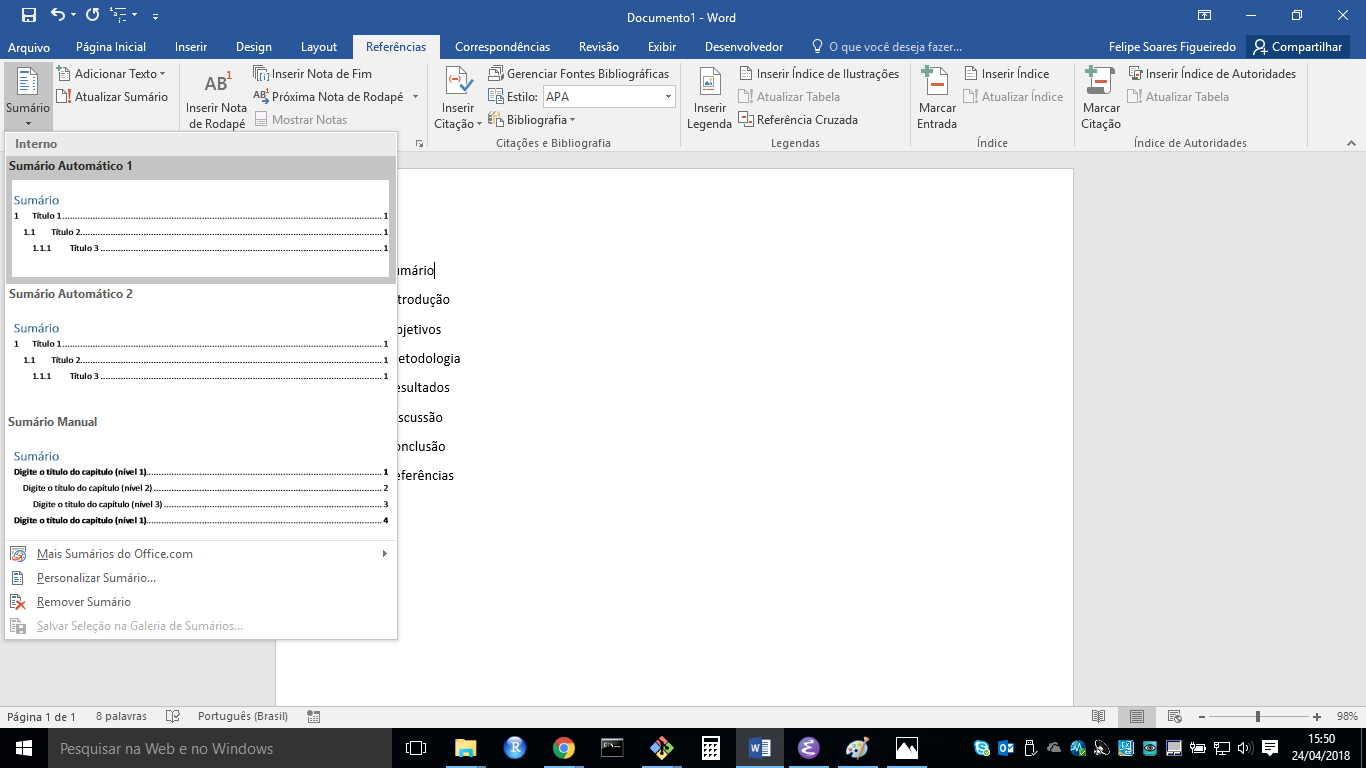
\includegraphics[height=0.9\textheight]{EstruturaII/sumario2}
\end{frame}

\begin{frame}{}
  \begin{block}{}
    \Large
    Vamos ver como se faz, na prática...
  \end{block}
\end{frame}

\section{Aprofundamento}

\subsection{Aprofundamento}

\begin{frame}{Aprofundamento}
  \begin{block}{Leitura obrigatória}
    Livro texto: capítulo {\bf 9} (Word)
  \end{block}
  \begin{block}{Leitura recomendada}
    \footnotesize
    Consultar, conforme necessidade: capítulos {\bf 6, 8}
  \end{block}
\end{frame}

% \section{Referências}

% \begin{frame}{Referências}
%   \begin{itemize}
%   \item<1-> VEduca:
%     \url{http://www.veduca.com.br/assistir/metodologia-cientifica}
%   % \item<1-> Prodanov (2013): cap 4.
%   % \item<1-> Lakatos (2003): cap 10.
%   \end{itemize}
% \end{frame}

\end{document}
